\subsection{CLASP and Cell Growth Model}

The data presented in Figure \ref{fig:mutant-sizes} along with similar data for atrichoblast cells was transformed into units of time and length using the following procedure. First, we make the assumption that cells are perfect cylinders, so that their surface area is related to their length by following formula:
$$\frac{A - 2\pi r^{2}}{2\pi r} = L$$

Then, we assume that the radius of each cell is identical, and prescribe a suitably chosen $r$ based on experimental data (\cite{goh2023}). To convert cell number to position we take the cumulative sum of the cell lengths over each cell column. Missing data was filled in using the average length for that cell number. Finally, we use the the function shown in Figure \ref{fig:position-function} to transform the position series into a time series and plot it against the cell lengths. The results of this data preprocessing is shown in Figures \ref{fig:data-trichoblast} and \ref{fig:data-atrichoblast} for trichoblast and atrichoblast cells respectively.

\begin{figure}[!hbt]
    \centering
    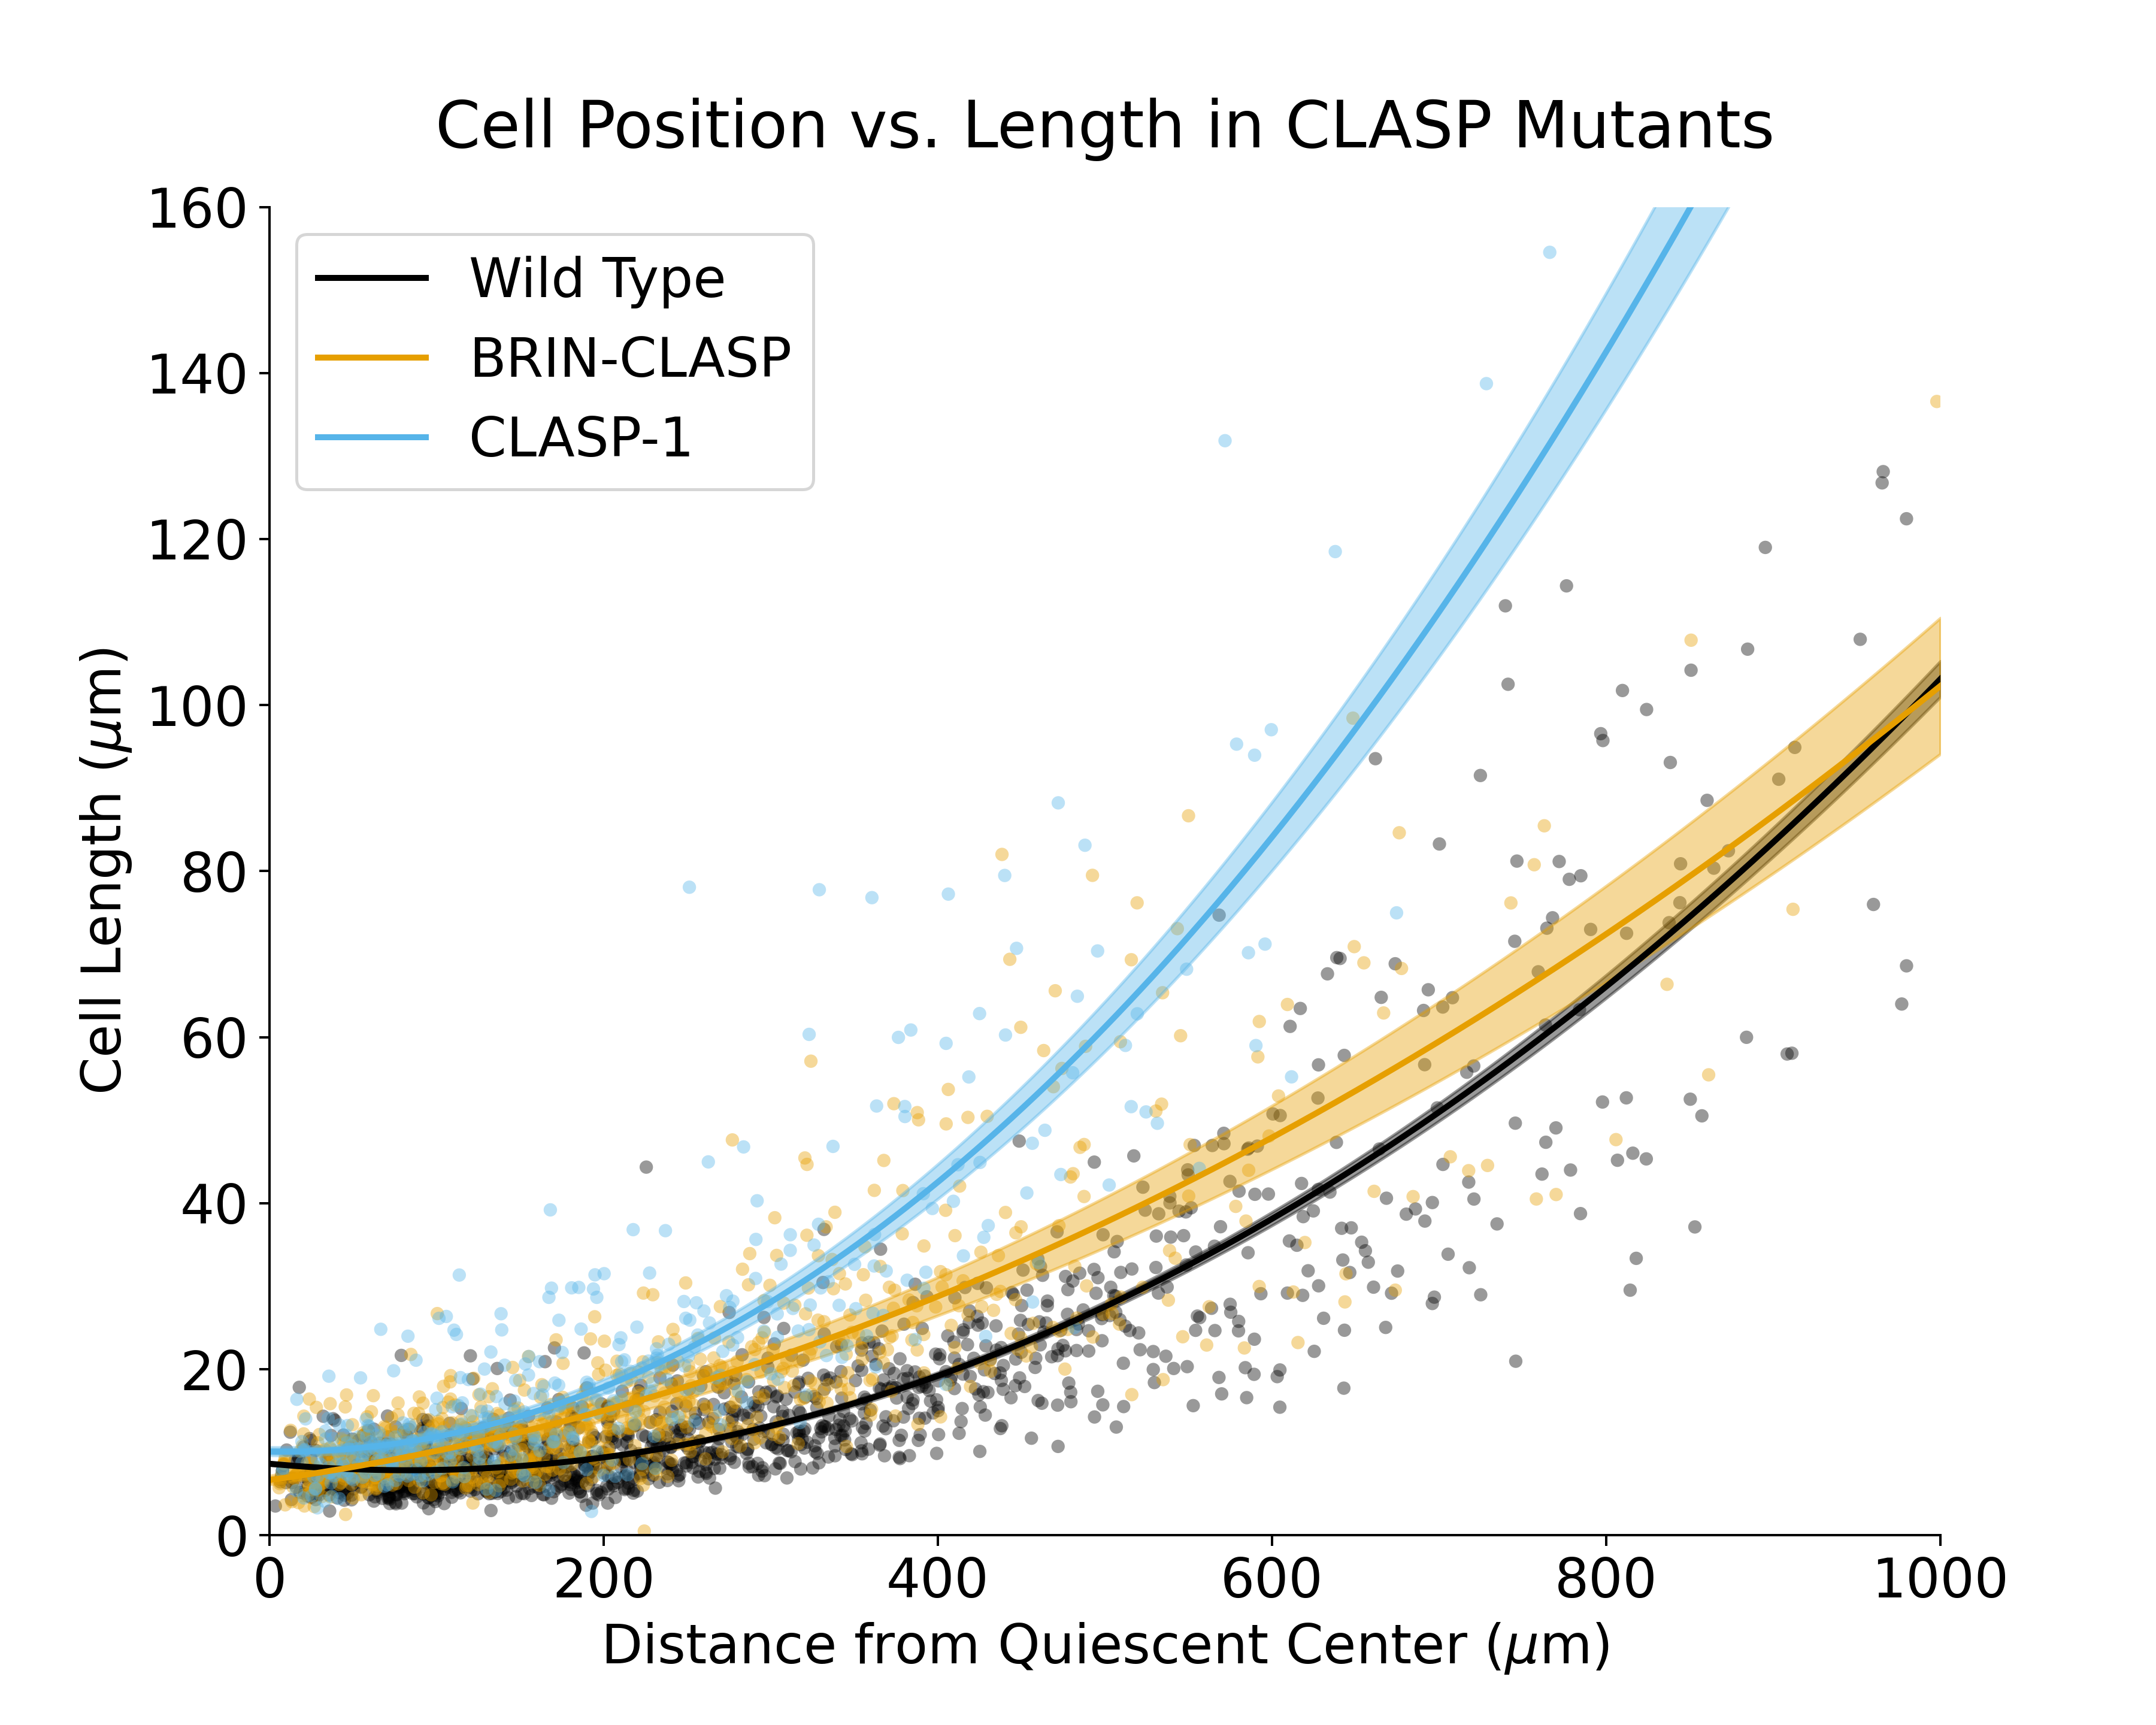
\includegraphics[width=13cm]{img/data-trichoblast.png}
    \caption{Plot of cell lengths from $N$ Wild Type, CLASP-1, and BRIN-CLASP roots. The line of best fit is an exponential function of the form $A + Be^{Cx}$. Wild Type cells are on average the shortest, followed closely by BRIN-CLASP. CLASP-1 cells are significantly longer, especially in the proximal regions of the root.}
    \label{fig:data-trichoblast}
\end{figure}

\begin{figure}[!hbt]
    \centering
    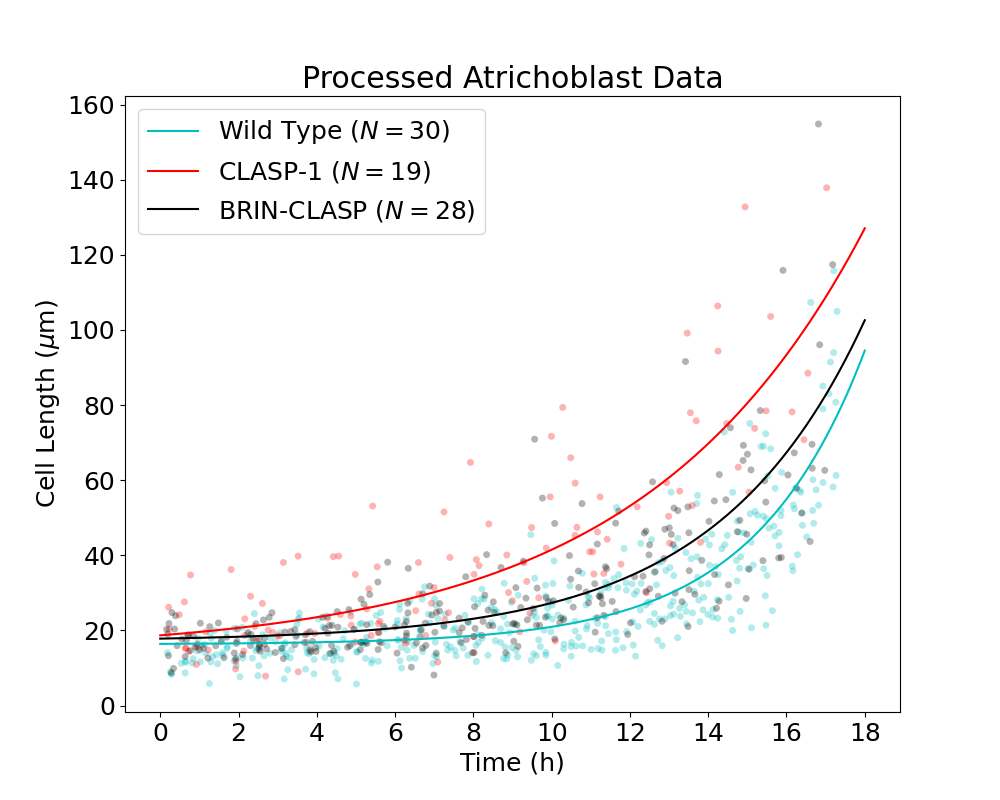
\includegraphics[width=13cm]{img/data-atrichoblast.png}
    \caption{Plot of cell lengths from $N$ Wild Type, CLASP-1, and BRIN-CLASP roots. The line of best fit is an exponential function of the form $A + Be^{Cx}$. Atrichoblast cells exhibit similar behaviour to trichoblast cells accross mutants, although atrichoblast cells are about $25\%$ longer.}
    \label{fig:data-atrichoblast}
\end{figure}

\medskip

For our first model of cell growth, we will consider exclusively wild type trichoblast cells. This model uses the ODE given in Equation \eqref{growth}, which is a variation on the model presented in \cite{lockhart1965} that accounts for the promotion of cell elongation by the BES1 transcription factor (\cite{vukasinovic2021}, \cite{ackerman-lavert2020}).

\begin{equation}
\label{growth}
\frac{dL}{dt} = (g_{P} + g_{B}\text{BES1})L
\end{equation}

In this model, $g_{P}$ denotes the basal growth rate due to the internal turgor pressure of the cell while $g_{B}$ denotes the rate at which $\text{BES1}$ promotes cell elongation. $\frac{dL}{dt}$ is scaled by the length $L$ because longer cells have more locations for the cellulose to stretch and reassemble (\cite{smithers2024}). An parameter corresponding to the initial condition $L(0) = g_{0}$ was also fitted. This parameter represents the average cell length at $150\um$ above the QC. 

\medskip

The BES1 equation \eqref{bes1} and length equation \eqref{growth} were approximated using a forward euler method with time step $0.01\ph$. Model fitting used the RMSE metric defined in equation \eqref{rmse} to fit the output to the data shown in Figure \ref{fig:data-trichoblast}. To reduce the dimensionality of the parameter space the parameters $s_{0}$, $s_{\text{in}}$, and $s_{\text{out}}$ from equation \eqref{bes1} were assigned their fitted values as shown in Figure \ref{fig:bes1-model-fit}. The parameter bounds used were $g_{0} \in [0, 10]$ and $g_{P}, g_{B} \in [0, 1]$. The results of the simulation are depicted in Figure \ref{fig:growth-model-fit}.

\begin{figure}[!hbt]
    \centering
    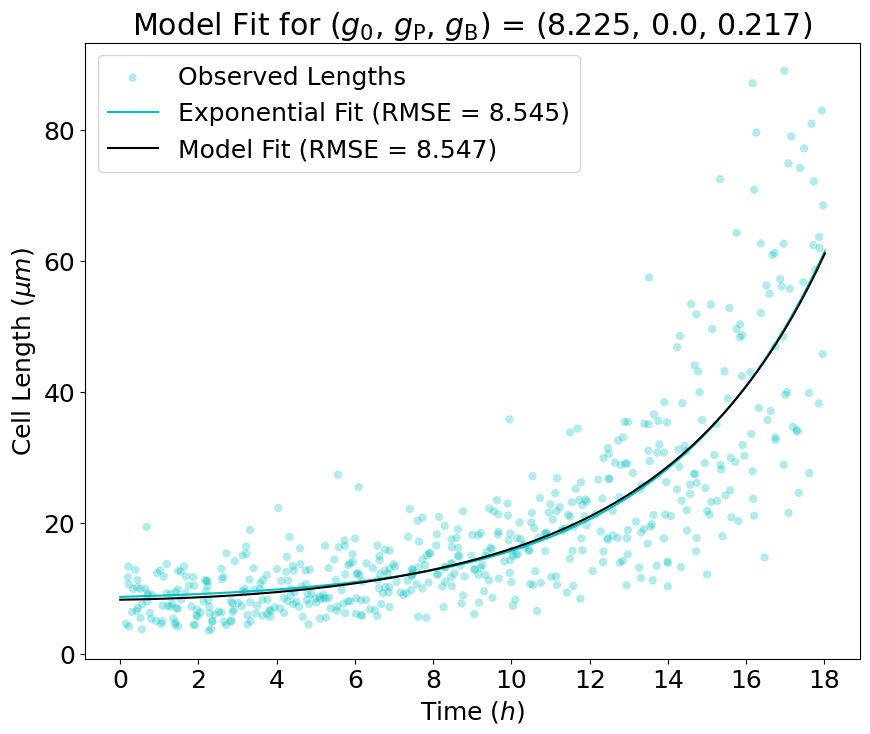
\includegraphics[width=13cm]{img/growth-model-fit.png}
    \caption{Results of fitting the growth model in equation \eqref{growth} to cell length data. The optimal parameter values were $g_{0} = 8.225\um$, $g_{P} = 0 \ph$ and $g_{B} = 0.0217\,\text{BES1}^{-1}\ph$. An exponential curve of the form $A + Be^{Cx}$ was also fitted to the data as a point of comparison. }
    \label{fig:growth-model-fit}
\end{figure}

\medskip

The result shown in Figure \ref{fig:growth-model-fit} suggests that our simple model is able to capture the trend in the data without invoking the existence of the CLASP protein. That being said, the abscence of the basal growth rate $g_{P}$ suggests that the optimal parameter values we found may not be representative of their true values. To get a better idea of the behaviour of our model we began by performing an uncertainty analysis. To do this, we  took each error $e_{i} = |f(t_{i}) - y_{i}|$, and then normalized it to get  the percentage error $\tilde{e_{i}} = e_{i} / y_{i}$. Then, we took the vectors of errors $\mathbf{e}$ and computed $1000$ random permutations $\mathbf{e}_{1}, \dots, \mathbf{e}_{1000}$. Finally, we constructed new $1000$ new data vectors $\mathbf{y}_{j} = f(\mathbf{t}) + \mathbf{e}_{j}$ and fitted the model to each one. The results of this analysis are shown in Figure \ref{fig:growth-model-uncertainty}.

\begin{figure}[!hbt]
    \centering
    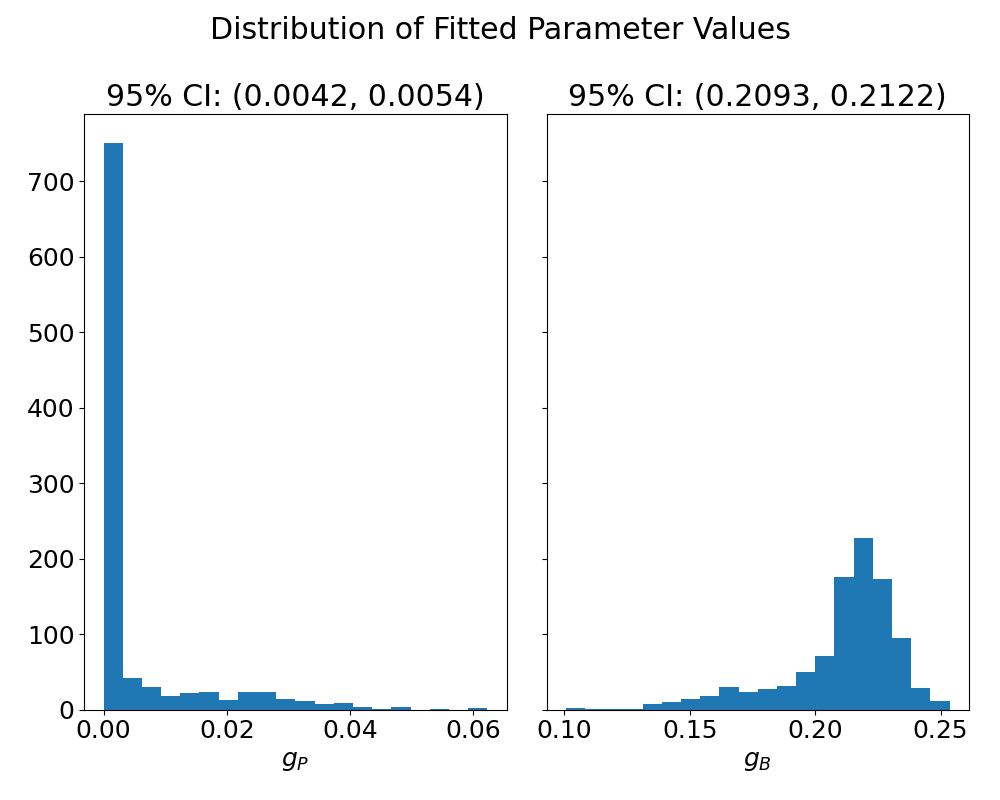
\includegraphics[width=13cm]{img/growth-model-uncertainty.png}
    \caption{A plot of the distribution of fitted $g_{P}$ and $g_{B}$ parameter values after the error shuffling process was repeated $1000$ times. Interestingly, the optimal parameters for the original data are outside the 95\% confidence intervals shown above. }
    \label{fig:growth-model-uncertainty}
\end{figure}

\medskip

A local sensitivity analysis over the domain $g_{P} \in [0, 0.1]$ and $g_{B} \in [0.1, 0.3]$ was also performed using the same methodologies described in Section \ref{bes1-model-section}. The results of this analysis are shown in Figure \ref{fig:growth-model-heatmap}.

\begin{figure}[!hbt]
    \centering
    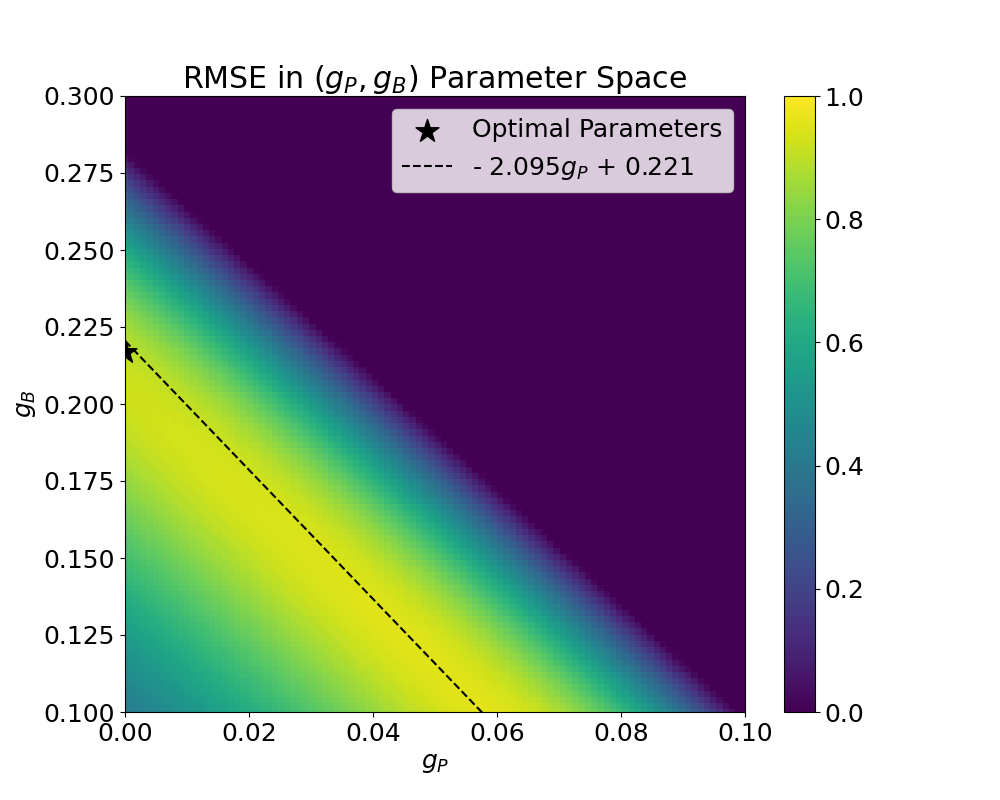
\includegraphics[width=13cm]{img/growth-model-heatmap.png}
    \caption{A heatmap of model error near the optimal parameter values $g_{P} = 0$ and $g_{B} = 0.217$. The RMSE remains low for values of $g_{B}$ and $g_{P}$ near the optimal range $g_{B} = -2.095g_{P} + 0.221$ but grows rapidly outside of that band. This result is not surprising given since if $g_{B}$ and $g_{P}$ are both high the model will overestimate the cell lengths. }
    \label{fig:growth-model-heatmap}
\end{figure}




